El proceso de pruebas para este proyecto se realizó a través de distintas etapas. De manera estática, se realizó la detección de las líneas del carril. En el proceso se encontró que la imagen recibía ruido procedente del color del suelo adyacente a la pista, lo cual fue posible mitigar al controlar las condiciones en las periferias del escenario. Otro error recurrente durante la detección del carril se obtiene cuando la cámara no se encuentra en una posición recta, provocando que sólo se detecte una de las líneas del carril.
\par La detección de los señalamientos de tránsito no es un proceso robusto, al contar sólo con una imagen para emparejamiento para cada señal. El algoritmo SURF aumenta sus costos computacionales cuando el emparejamiento toma un número mayor de imágenes objeto, lo cual dificulta al vehículo identificar los señalamientos por el tiempo que toma a la computadora procesar la información. Como desventaja de emplear sólo una imagen objeto para cada señal, es que la si la inclinación del plano del señalamiento tiene una apertura amplia con respecto al plano del vehículo, entonces la adquisición y comparación de descriptores no es existosa y, por lo tanto, el vehículo no detecta el señalamiento. En el par de imágenes de la Figura \ref{fig:SSURF} se muestran emparejamientos correctos con el algoritmo.
\begin{figure}[htbp!]
	\centering
	\begin{subfigure}[htbp!]{0.4\textwidth}
		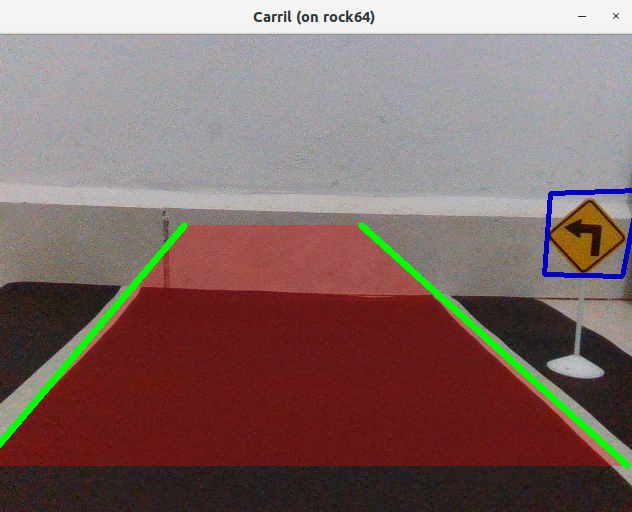
\includegraphics[width=\textwidth]{./Figuras/SSURF1}
	\end{subfigure}
	\begin{subfigure}[htbp!]{0.4\textwidth}
		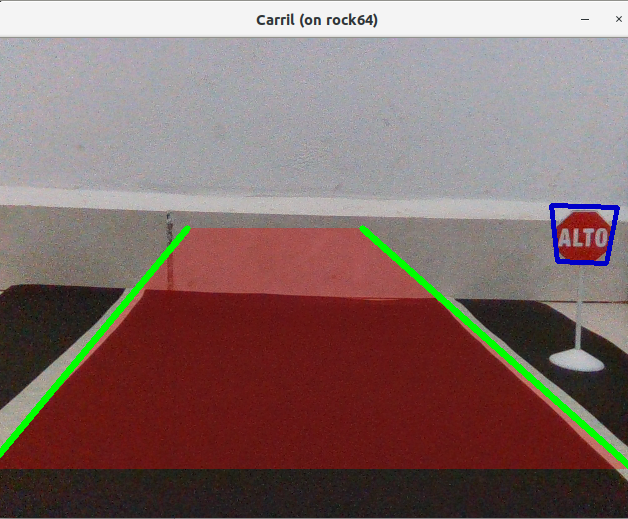
\includegraphics[width=\textwidth]{./Figuras/SSURF2}
	\end{subfigure}
	\caption{Emparejamientos positivos con el algoritmo SURF.}
	\label{fig:SSURF}
\end{figure}
\par Por su cuenta, en el par de impágenes de la Figura \ref{fig:NSURF} se muestran emparejamientos nulos con el algoritmo, estos se deben a la orientación del señalamiento en la imagen.
\begin{figure}[htbp!]
	\centering
	\begin{subfigure}[htbp!]{0.4\textwidth}
		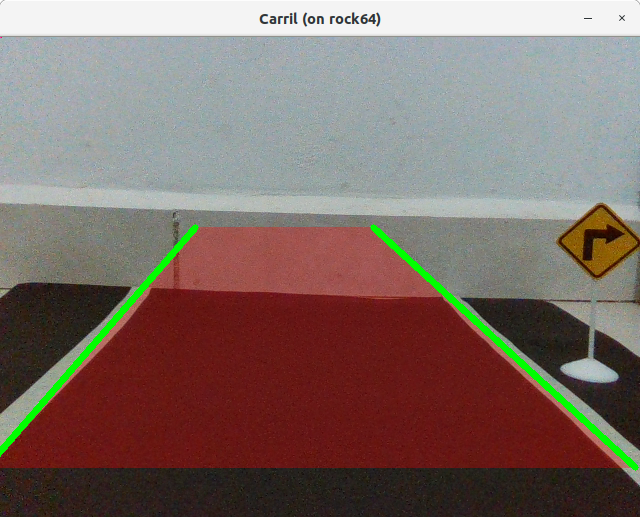
\includegraphics[width=\textwidth]{./Figuras/NSURF1}
	\end{subfigure}
	\begin{subfigure}[htbp!]{0.4\textwidth}
		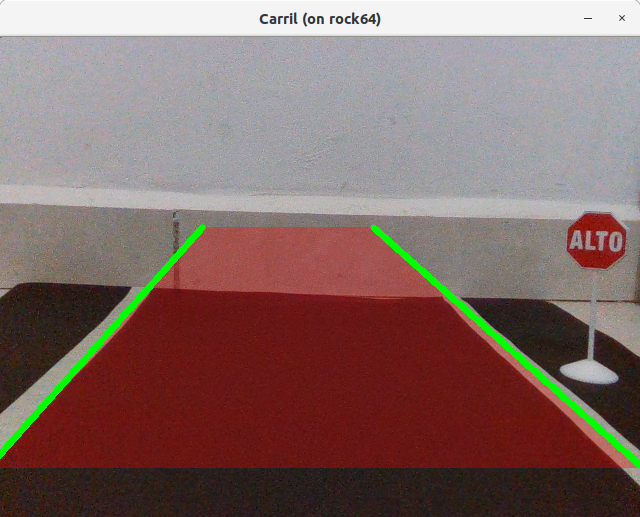
\includegraphics[width=\textwidth]{./Figuras/NSURF2}
	\end{subfigure}
	\caption{Emparejamientos nulos con el algoritmo SURF.}
	\label{fig:NSURF}
\end{figure}
\par Por último, para seguir la navegación del vehículo durante todo su recorrido se implementó la odometría visual basado en descriptores FAST. Las funciones concernientes a la odometría visual están presentes en la clase Navegación. Como resultado de esta implementación, en la Figura \ref{fig:odom} se muestra la salida del programa para dos pruebas en las que el programa trabajó {\it fuera de línea}; el programa devuelve una ventana de 300x300 pixeles que representa un escenario de 3x3 m. En la ventana se observa a lo largo del tiempo cómo se dibujan nuevos puntos azules, indicando de manera aproximada el camino recorrido por el vehículo desde su configuración inicial a su configuración final.
\begin{figure}[htbp!]
	\centering
	\begin{subfigure}[htbp!]{0.4\textwidth}
		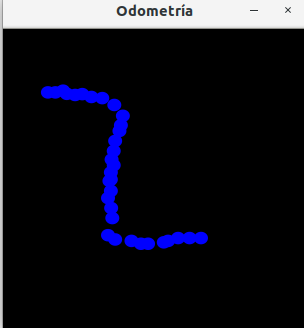
\includegraphics[width=\textwidth]{./Figuras/Odo1}
	\end{subfigure}
	\begin{subfigure}[htbp!]{0.4\textwidth}
		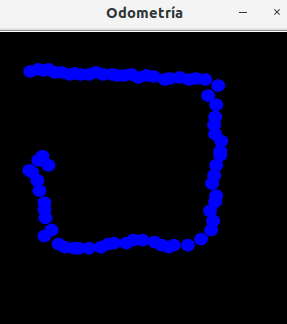
\includegraphics[width=\textwidth]{./Figuras/Odo2}
	\end{subfigure}
	\caption{Seguimiento de la trayectoria del vehículo a través de odometría visual.}
	\label{fig:odom}
\end{figure}
\par Estas imágenes finales correspondientes a la odometría, por su caracter de trabajo extra, no se encuentran documentadas en su totalidad, y en la Sección de trabajo futuro se establece que se continuará trabajando en este elemento.